\PassOptionsToPackage{unicode=true}{hyperref} % options for packages loaded elsewhere
\PassOptionsToPackage{hyphens}{url}
%
\documentclass[]{article}
\usepackage{lmodern}
\usepackage{amssymb,amsmath}
\usepackage{ifxetex,ifluatex}
\usepackage{fixltx2e} % provides \textsubscript
\ifnum 0\ifxetex 1\fi\ifluatex 1\fi=0 % if pdftex
  \usepackage[T1]{fontenc}
  \usepackage[utf8]{inputenc}
  \usepackage{textcomp} % provides euro and other symbols
\else % if luatex or xelatex
  \usepackage{unicode-math}
  \defaultfontfeatures{Ligatures=TeX,Scale=MatchLowercase}
\fi
% use upquote if available, for straight quotes in verbatim environments
\IfFileExists{upquote.sty}{\usepackage{upquote}}{}
% use microtype if available
\IfFileExists{microtype.sty}{%
\usepackage[]{microtype}
\UseMicrotypeSet[protrusion]{basicmath} % disable protrusion for tt fonts
}{}
\IfFileExists{parskip.sty}{%
\usepackage{parskip}
}{% else
\setlength{\parindent}{0pt}
\setlength{\parskip}{6pt plus 2pt minus 1pt}
}
\usepackage{hyperref}
\hypersetup{
            pdftitle={Is Sans Forgetica Really Unforgettable?},
            pdfborder={0 0 0},
            breaklinks=true}
\urlstyle{same}  % don't use monospace font for urls
\usepackage[margin=1in]{geometry}
\usepackage{color}
\usepackage{fancyvrb}
\newcommand{\VerbBar}{|}
\newcommand{\VERB}{\Verb[commandchars=\\\{\}]}
\DefineVerbatimEnvironment{Highlighting}{Verbatim}{commandchars=\\\{\}}
% Add ',fontsize=\small' for more characters per line
\usepackage{framed}
\definecolor{shadecolor}{RGB}{248,248,248}
\newenvironment{Shaded}{\begin{snugshade}}{\end{snugshade}}
\newcommand{\AlertTok}[1]{\textcolor[rgb]{0.94,0.16,0.16}{#1}}
\newcommand{\AnnotationTok}[1]{\textcolor[rgb]{0.56,0.35,0.01}{\textbf{\textit{#1}}}}
\newcommand{\AttributeTok}[1]{\textcolor[rgb]{0.77,0.63,0.00}{#1}}
\newcommand{\BaseNTok}[1]{\textcolor[rgb]{0.00,0.00,0.81}{#1}}
\newcommand{\BuiltInTok}[1]{#1}
\newcommand{\CharTok}[1]{\textcolor[rgb]{0.31,0.60,0.02}{#1}}
\newcommand{\CommentTok}[1]{\textcolor[rgb]{0.56,0.35,0.01}{\textit{#1}}}
\newcommand{\CommentVarTok}[1]{\textcolor[rgb]{0.56,0.35,0.01}{\textbf{\textit{#1}}}}
\newcommand{\ConstantTok}[1]{\textcolor[rgb]{0.00,0.00,0.00}{#1}}
\newcommand{\ControlFlowTok}[1]{\textcolor[rgb]{0.13,0.29,0.53}{\textbf{#1}}}
\newcommand{\DataTypeTok}[1]{\textcolor[rgb]{0.13,0.29,0.53}{#1}}
\newcommand{\DecValTok}[1]{\textcolor[rgb]{0.00,0.00,0.81}{#1}}
\newcommand{\DocumentationTok}[1]{\textcolor[rgb]{0.56,0.35,0.01}{\textbf{\textit{#1}}}}
\newcommand{\ErrorTok}[1]{\textcolor[rgb]{0.64,0.00,0.00}{\textbf{#1}}}
\newcommand{\ExtensionTok}[1]{#1}
\newcommand{\FloatTok}[1]{\textcolor[rgb]{0.00,0.00,0.81}{#1}}
\newcommand{\FunctionTok}[1]{\textcolor[rgb]{0.00,0.00,0.00}{#1}}
\newcommand{\ImportTok}[1]{#1}
\newcommand{\InformationTok}[1]{\textcolor[rgb]{0.56,0.35,0.01}{\textbf{\textit{#1}}}}
\newcommand{\KeywordTok}[1]{\textcolor[rgb]{0.13,0.29,0.53}{\textbf{#1}}}
\newcommand{\NormalTok}[1]{#1}
\newcommand{\OperatorTok}[1]{\textcolor[rgb]{0.81,0.36,0.00}{\textbf{#1}}}
\newcommand{\OtherTok}[1]{\textcolor[rgb]{0.56,0.35,0.01}{#1}}
\newcommand{\PreprocessorTok}[1]{\textcolor[rgb]{0.56,0.35,0.01}{\textit{#1}}}
\newcommand{\RegionMarkerTok}[1]{#1}
\newcommand{\SpecialCharTok}[1]{\textcolor[rgb]{0.00,0.00,0.00}{#1}}
\newcommand{\SpecialStringTok}[1]{\textcolor[rgb]{0.31,0.60,0.02}{#1}}
\newcommand{\StringTok}[1]{\textcolor[rgb]{0.31,0.60,0.02}{#1}}
\newcommand{\VariableTok}[1]{\textcolor[rgb]{0.00,0.00,0.00}{#1}}
\newcommand{\VerbatimStringTok}[1]{\textcolor[rgb]{0.31,0.60,0.02}{#1}}
\newcommand{\WarningTok}[1]{\textcolor[rgb]{0.56,0.35,0.01}{\textbf{\textit{#1}}}}
\usepackage{longtable,booktabs}
% Fix footnotes in tables (requires footnote package)
\IfFileExists{footnote.sty}{\usepackage{footnote}\makesavenoteenv{longtable}}{}
\usepackage{graphicx,grffile}
\makeatletter
\def\maxwidth{\ifdim\Gin@nat@width>\linewidth\linewidth\else\Gin@nat@width\fi}
\def\maxheight{\ifdim\Gin@nat@height>\textheight\textheight\else\Gin@nat@height\fi}
\makeatother
% Scale images if necessary, so that they will not overflow the page
% margins by default, and it is still possible to overwrite the defaults
% using explicit options in \includegraphics[width, height, ...]{}
\setkeys{Gin}{width=\maxwidth,height=\maxheight,keepaspectratio}
\setlength{\emergencystretch}{3em}  % prevent overfull lines
\providecommand{\tightlist}{%
  \setlength{\itemsep}{0pt}\setlength{\parskip}{0pt}}
\setcounter{secnumdepth}{0}
% Redefines (sub)paragraphs to behave more like sections
\ifx\paragraph\undefined\else
\let\oldparagraph\paragraph
\renewcommand{\paragraph}[1]{\oldparagraph{#1}\mbox{}}
\fi
\ifx\subparagraph\undefined\else
\let\oldsubparagraph\subparagraph
\renewcommand{\subparagraph}[1]{\oldsubparagraph{#1}\mbox{}}
\fi

% set default figure placement to htbp
\makeatletter
\def\fps@figure{htbp}
\makeatother


\title{Is Sans Forgetica Really Unforgettable?}
\author{}
\date{\vspace{-2.5em}}

\begin{document}
\maketitle

\textless{}\textless{}\textless{}\textless{}\textless{}\textless{}\textless{}
HEAD The primary goal of most humans is to remember the information they
lean. Decades of research have put forth the paradoxical idea that
making learning harder (not easier) should have the desirable effect of
improving long-term retention of material--called the desirable
diffuclty principle (Bjork, 1994). Notable examples of desirable
difficulties include having participants generate information from word
fragments instead of passively reading intact words (e.g., Slamecka \&
Graf, 1978), spacing out study sessions instead of massing them (e.g.,
Carpenter, 2017), and having participants engage in retrieval practice
after studying instead of simply restudying the information (Kornell \&
Vaughn, 2016). Another simple strategy that has gained some attention is
to make material more perceptually disfluent. This can be done by
changing the material's perceptual characteristics (Diemand-Yaumen,
Oppenheimer, \& Vaughan, 2011; French et al., 2013). Visual material
that is masked (Mulligan, ======= Stundents want to remmeber the
information they lean. Decades of research have put forth the
paradoxical idea that making learning harder (not easier) should have
the desirable effect of improving long-term retention of
material--called the desirable diffuclty principle (Bjork, 1994).
Notable examples of desirable difficulties include having participants
generate information from word fragments instead of passively reading
intact words (e.g., Slamecka \& Graf, 1978), spacing out study sessions
instead of massing them (e.g., Carpenter, 2017), and having participants
engage in retrieval practice after studying instead of simply restudying
the information (Kornell \& Vaughn, 2016). Another simple strategy that
has gained some attention is to make material more perceptually
disfluent. This can be done by changing the material's perceptual
characteristics (Diemand-Yaumen, Oppenheimer, \& Vaughan, 2011; French
et al., 2013). Visual material that is masked (Mulligan,
\textgreater{}\textgreater{}\textgreater{}\textgreater{}\textgreater{}\textgreater{}\textgreater{}
12407944d8d1cb604995f74327fa48b59136590f 1996), inverted (Sungkhasette,
Friedman, \& Castel, 2011), presented in an atypical font (Diemand
Yaumen et al., 2011), blurred (Rosner, Davis, \& Milliken, 2015), or
even in handwritten cursive (Geller, Still, Dark, Carpenter, 2018) have
all been shown to produce memory benefits. The desirable effect of
perceptual disfluency on memory is called called the disfluency effect.

Although appealing as a pedagogical strategy, there have been several
experiments that failed to find memorial benefits for perceptually
disfluent materials (e.g., Magreehan, Serra, Schwartz \& Narciss, 2016;
Rhodes \& Castel, 2008, 2009; Rummer, Scheweppe, \& Schewede, 2016; Yue,
Castel, \& Bjork, 2013), casting doubt upon the veracity of the
disfluency effect. Recent studies by Geller et al.(2018) and Geller \&
Still (2018) found that perceptual disfluency can have a beneficial
effect on memory, but seems to be rather fickle, thus delimiting its
educational usefuleness.

\textless{}\textless{}\textless{}\textless{}\textless{}\textless{}\textless{}
HEAD Given the weak evidence, it came as a surprise to me when a little
over a year ago, I saw a font by the name of Sans Forgetica (SF) getting
a ton of press coverage. The mnnmenomic benefits of this font,
\emph{based on cognitive psychology}, were being touted in reputable
news sources like Washington Post
(\url{https://www.washingtonpost.com/business/2018/10/05/introducing-sans-forgetica-font-designed-boost-your-memory/})
and NPR
(\url{https://www.npr.org/2018/10/06/655121384/sans-forgetica-a-font-to-remember},
amongst others. The creators even made the SF font available for mac and
pc operating systems--all you have to do is downlaod the font file and
you to can remember everything you read :). There is even a Chrome
browser extension and cellphone application that allows users to place
material in Sans Forgetica. With this much attention and marketing,
there has to be solid empirical evidence backing it up, right? Not
quite. ======= Despite the weak evidence for perceptual disfluency, it
came as a surprise to me when a little over a year ago, I saw a font by
the name of Sans Forgetica (SF) getting a ton of press coverage. The
mnnmenomic benefits of this font, \emph{based on cognitive psychology},
were being touted in reputable news sources like Washington Post
(\url{https://www.washingtonpost.com/business/2018/10/05/introducing-sans-forgetica-font-designed-boost-your-memory/})
and NPR
(\url{https://www.npr.org/2018/10/06/655121384/sans-forgetica-a-font-to-remember},
amongst others. The creators even made the SF font available for mac and
pc operating systems--all you have to do is downlaod the font file and
you to can remember everything you read :). There is even a Chrome
browser extension and cellphone application that allows users to place
material in Sans Forgetica. With this much attention and marketing,
there has to be solid empirical evidence backing it up, right? Not
quite.
\textgreater{}\textgreater{}\textgreater{}\textgreater{}\textgreater{}\textgreater{}\textgreater{}
12407944d8d1cb604995f74327fa48b59136590f

\hypertarget{what-do-we-know-about-sf}{%
\section{What do we know about SF?}\label{what-do-we-know-about-sf}}

There is not information about SF. The typyface itself is a variation of
a sans-serif typeface. It is a typeface that consists of intermitten
gaps in letters that are back slanted (see below picture). The design
features of this typeface require readers of it to ``fill-in'' the
missing pieces like a puzzle. As it pertains to the empirical validation
of the claims made, the website does offer some information about SF and
how the original results were obtained, but not enough information to
replicate the studies.

\begin{figure}
\centering
\includegraphics{https://user-images.githubusercontent.com/18429968/70854186-006bd180-1e7e-11ea-8fe1-94f5cf37c805.png}
\caption{image}
\end{figure}

\textless{}\textless{}\textless{}\textless{}\textless{}\textless{}\textless{}
HEAD Earp (2018) conducted an interview with the creators of SF and here
is what we know. Apparently two studies were conducted. In a lab
experiment (\emph{N}=96), they had participants read 20 word pairs
(e.g., girl - guy; called a paried associates task in cognitive
parlance) in three new fonts (one of them being SF) and a typical or
common font. The font pairs were presented were counterbalanced across
participants. What this means is that all fonts were shown, but the same
pairs were never presneted in more than one type of font. Each word pair
was presnted on the screen for 100 ms (that is super fast\ldots{}). For
a final test, they were given the cue (e.g., \emph{girl}) and had to
respond with the target (\emph{guy}). What did they find? According to
the interview, targets were recalled 68\% of time when presented in a
common font. For cue-target pairs in SF, targets were recalled 69\% of
the time--a negeliable difference. ======= Earp (2018) conducted an
interview with the creators of SF and I was able to glean some details
about how SF ws validated. Apparently two studies were conducted. In a
lab experiment (\emph{N}=96), they had participants read 20 word pairs
(e.g., girl - guy; called a paried associates task in cognitive
parlance) in three new fonts (one of them being SF) and a typical or
common font. The font pairs were presented in was counterbalanced
participants. What this means is that all fonts were showns, but the
same pairs were never presneted in more than one type of font. Each word
pair was presnted on the screen for 100 ms (that is super fast\ldots{}).
For a final test, they were given the cue (e.g., \emph{girl}) and had to
respond with the target (\emph{guy}). What did they find? According to
the interview, targets were recalled 68\% of time when presented in a
common font. For cue-target pairs in SF, targets were recalled 69\% of
the time--a negeliable difference.
\textgreater{}\textgreater{}\textgreater{}\textgreater{}\textgreater{}\textgreater{}\textgreater{}
12407944d8d1cb604995f74327fa48b59136590f

In an online experiment, participants were presented passages (250 words
in total) where one of the paragraphs was presented in SF. Each
participant saw five different texts in total. For each text they were
asked one question about the part written in SF and another question
about the part written in standard Arial. Participants remembered 57\%
of the text when a section was written in Sans Forgetica, compared to
50\% of the surrounding text that was written in a plain Arial font.

At the time of this writing, these studies have not been published nor
is there a preprint available. I reached out to the creators of SF, but
they refused to share the materials with me. Instead of waiting, I
elicited the help of Sara Davis and Daniel Peterson at Skidmore
university to test the mnenmomic benefits of Sans Forgetica. We
preregistered two studies (\url{https://osf.io/d2vy8/}). All materials,
data, and analysis scripts can be found at that website. On my github,
you can reproduce all analyses for the two reported experiments in an
online container (\url{https://github.com/jgeller112/SF_Expt1};
\url{https://github.com/jgeller112/SF_Expt2}).

\hypertarget{experiment-1}{%
\section{Experiment 1}\label{experiment-1}}

In the first study we compared the mnenmonic benefits of SF against a
robust technique known to enhance memory---generation. The generation
effect is a phenomenon where information is better remembered when
retrieved than if it is simply read. In a prototypical
experiment,participants are asked to generate words from word fragments
DOLL - DR\_\_ or read intact cue-target pairs (\emph{DOLL-DRESS}).
Compared to the intact condition, individuals recall the generated
target words at a higher rate. The natural of generation is where the
power of SF comes from, according to the authors. We put that to the
test in the first experiment.

\textless{}\textless{}\textless{}\textless{}\textless{}\textless{}\textless{}
HEAD We preregistered a sample size of 230 participants (115 per group)
to detect a small-to medium size interaction effect (d = .35) with 90\%
power. We choose this effect size as our SESOI due in part due the small
effect sizes seen in actaul classroom studies (Bulter et al., 2014). We
recruited 230 people from Amazon's Mechanical Turk Service. We initially
collected data from 120 people, and then excluded participants who 1)
did not complete every phase of the experiment, 2) started the
experiment multiple times, 3) reported experiencing technical problems
did not indicate that they were fluent in English, or 5) reported seeing
our stimuli before.

\hypertarget{in-experiment-1-participants-were-presented-with-40-weakly-related-cue-target-pairs.-the-pairs-were-all-nouns-57-letters-and-13-syllables-in-length-and-high-in-concreteness-400700-and-frequency-at-least-30-per-million.-for-half-of-the-participants-half-of-the-targets-were-presented-in-sf-while-the-other-half-were-presented-in-arial-font-for-the-other-half-of-participants-the-targets-were-presented-with-missing-letters-vowels-were-replaced-by-underscores-and-the-other-half-were-intact-arial-font.-after-a-short-2-minute-distractor-task-anagram-generation-they-completed-a-cued-recall-test.}{%
\section{In Experiment 1 participants were presented with 40 weakly
related cue-target pairs. The pairs were all nouns, 5--7 letters and
1--3 syllables in length, and high in concreteness (400--700) and
frequency (at least 30 per million). For half of the participants, half
of the targets were presented in SF while the other half were presented
in Arial font; for the other half of participants, the targets were
presented with missing letters (vowels were replaced by underscores) and
the other half were intact (Arial font). After a short 2 minute
distractor task (anagram generation), they completed a cued recall
test.}\label{in-experiment-1-participants-were-presented-with-40-weakly-related-cue-target-pairs.-the-pairs-were-all-nouns-57-letters-and-13-syllables-in-length-and-high-in-concreteness-400700-and-frequency-at-least-30-per-million.-for-half-of-the-participants-half-of-the-targets-were-presented-in-sf-while-the-other-half-were-presented-in-arial-font-for-the-other-half-of-participants-the-targets-were-presented-with-missing-letters-vowels-were-replaced-by-underscores-and-the-other-half-were-intact-arial-font.-after-a-short-2-minute-distractor-task-anagram-generation-they-completed-a-cued-recall-test.}}

In Experiment 1 we had 115 particpants in each condition (\emph{N} =
230). Data was collected using MTurk. We preregistered a sample size of
230 participants (115 per group) to detect a small-to medium size
interaction effect (d = .35) with 90\% power. We choose this effect size
as our SESOI due in part due the small effect sizes seen in actaul
classroom studies (Bulter et al., 2014).

In Experiment 1 participants were presented with 40 weakly
relatedcue-targte pairs. The pairs were nouns, 5--7 letters, 1--3
syllables in length, and high in concreteness (400--700) and frequency
(at least 30 per million). For half of the participants, half of the
targets were presented in SF while the other half were presented in
Arial font; for the other half of participants, the targets were
presented with missing letters (vowels were replaced by underscores) and
the other half were intact (Arial font). After a short 2 minute
distractor task (anagram generation), they completed a cued recall test.

Spell checking was automated with the hunspell package in R (Ooms, 2018)
using spellCheck.R. Becasuse participants were recruited in the United
States, we used the American English dictionary. A nice walkthrough on
how to use the package can be found in Buchcamam, De Deyne, \&
Montefinese (2019). Using the package, each response was corrected for
misspelings. Corrected spellings are provided in the most probable
order, therefore, the first suggestion is selected as the correct
answer. Answers were marked correct if they provided the exact response.
\textgreater{}\textgreater{}\textgreater{}\textgreater{}\textgreater{}\textgreater{}\textgreater{}
12407944d8d1cb604995f74327fa48b59136590f

In order for a response to be judged correctly, the response had to
match the correct answer. Scoring was automated with the hunspell
package in R (Ooms, 2018). Using the package, each response was
corrected for misspelings. Becasuse participants were recruited in the
United States, we used the American English dictionary. A nice
walkthrough on how to use the package can be found in Buchcamam, De
Deyne, \& Montefinese (2019). The most probably response (the first
answer) was chosen as the correct spelling. What did we find?

In Experiment 1 we found a sizeable generation effect, which replicated
past work. However, we did not find a SF effect (See figure below)

\begin{Shaded}
\begin{Highlighting}[]
\KeywordTok{library}\NormalTok{(qualtRics)}
\KeywordTok{library}\NormalTok{(tidyverse)}
\end{Highlighting}
\end{Shaded}

\begin{verbatim}
## ── Attaching packages ──────────────────────────────────────────── tidyverse 1.3.0 ──
\end{verbatim}

\begin{verbatim}
## ✓ ggplot2 3.2.1     ✓ purrr   0.3.3
## ✓ tibble  2.1.3     ✓ dplyr   0.8.3
## ✓ tidyr   1.0.0     ✓ stringr 1.4.0
## ✓ readr   1.3.1     ✓ forcats 0.4.0
\end{verbatim}

\begin{verbatim}
## ── Conflicts ─────────────────────────────────────────────── tidyverse_conflicts() ──
## x dplyr::filter() masks stats::filter()
## x dplyr::lag()    masks stats::lag()
\end{verbatim}

\begin{Shaded}
\begin{Highlighting}[]
\KeywordTok{library}\NormalTok{(afex)}
\end{Highlighting}
\end{Shaded}

\begin{verbatim}
## Loading required package: lme4
\end{verbatim}

\begin{verbatim}
## Loading required package: Matrix
\end{verbatim}

\begin{verbatim}
## 
## Attaching package: 'Matrix'
\end{verbatim}

\begin{verbatim}
## The following objects are masked from 'package:tidyr':
## 
##     expand, pack, unpack
\end{verbatim}

\begin{verbatim}
## Registered S3 methods overwritten by 'car':
##   method                          from
##   influence.merMod                lme4
##   cooks.distance.influence.merMod lme4
##   dfbeta.influence.merMod         lme4
##   dfbetas.influence.merMod        lme4
\end{verbatim}

\begin{verbatim}
## ************
## Welcome to afex. For support visit: http://afex.singmann.science/
\end{verbatim}

\begin{verbatim}
## - Functions for ANOVAs: aov_car(), aov_ez(), and aov_4()
## - Methods for calculating p-values with mixed(): 'KR', 'S', 'LRT', and 'PB'
## - 'afex_aov' and 'mixed' objects can be passed to emmeans() for follow-up tests
## - NEWS: library('emmeans') now needs to be called explicitly!
## - Get and set global package options with: afex_options()
## - Set orthogonal sum-to-zero contrasts globally: set_sum_contrasts()
## - For example analyses see: browseVignettes("afex")
## ************
\end{verbatim}

\begin{verbatim}
## 
## Attaching package: 'afex'
\end{verbatim}

\begin{verbatim}
## The following object is masked from 'package:lme4':
## 
##     lmer
\end{verbatim}

\begin{Shaded}
\begin{Highlighting}[]
\KeywordTok{library}\NormalTok{(emmeans)}
\end{Highlighting}
\end{Shaded}

\begin{verbatim}
## Welcome to emmeans.
## NOTE -- Important change from versions <= 1.41:
##     Indicator predictors are now treated as 2-level factors by default.
##     To revert to old behavior, use emm_options(cov.keep = character(0))
\end{verbatim}

\begin{Shaded}
\begin{Highlighting}[]
\KeywordTok{library}\NormalTok{(here)}
\end{Highlighting}
\end{Shaded}

\begin{verbatim}
## here() starts at /Users/gellr/SF_Expt2
\end{verbatim}

\begin{Shaded}
\begin{Highlighting}[]
\KeywordTok{library}\NormalTok{(ggpol)}
\KeywordTok{library}\NormalTok{(knitr)}
\NormalTok{sfgen1<-}\KeywordTok{read_csv}\NormalTok{(}\StringTok{"expt1agg1.csv"}\NormalTok{)}
\end{Highlighting}
\end{Shaded}

\begin{verbatim}
## Warning: Missing column names filled in: 'X1' [1]
\end{verbatim}

\begin{verbatim}
## Parsed with column specification:
## cols(
##   X1 = col_double(),
##   ResponseID = col_character(),
##   condition = col_character(),
##   dis = col_character(),
##   accuracy = col_double()
## )
\end{verbatim}

\begin{Shaded}
\begin{Highlighting}[]
\CommentTok{## get aggreagte recall per subject, condition, and dis}

\NormalTok{sfgenagg <-}\StringTok{ }\NormalTok{sfgen1 }\OperatorTok\StringTok{ }
\StringTok{  }\NormalTok{dplyr}\OperatorTok{::}\KeywordTok{group_by}\NormalTok{(ResponseID, condition, dis) }\OperatorTok
\StringTok{  }\NormalTok{dplyr}\OperatorTok{::}\KeywordTok{summarise}\NormalTok{(}\DataTypeTok{accuracy=}\KeywordTok{mean}\NormalTok{(accuracy))}

\CommentTok{#perform mixed ANOVA}
\NormalTok{a1 <-}\StringTok{ }\KeywordTok{aov_ez}\NormalTok{(}\StringTok{"ResponseID"}\NormalTok{, }\StringTok{"accuracy"}\NormalTok{, sfgenagg, }
             \DataTypeTok{within =} \KeywordTok{c}\NormalTok{(}\StringTok{"dis"}\NormalTok{), }\DataTypeTok{between =} \KeywordTok{c}\NormalTok{(}\StringTok{"condition"}\NormalTok{)) }\CommentTok{# 2 X 2 Mixed ANOVA}
\end{Highlighting}
\end{Shaded}

\begin{verbatim}
## Converting to factor: condition
\end{verbatim}

\begin{verbatim}
## Contrasts set to contr.sum for the following variables: condition
\end{verbatim}

\begin{Shaded}
\begin{Highlighting}[]
\CommentTok{#plot the results}

\KeywordTok{kable}\NormalTok{(}\KeywordTok{nice}\NormalTok{(a1))}
\end{Highlighting}
\end{Shaded}

\begin{longtable}[]{@{}llllll@{}}
\toprule
Effect & df & MSE & F & ges & p.value\tabularnewline
\midrule
\endhead
condition & 1, 230 & 0.10 & 0.00 & \textless{}.0001 & .99\tabularnewline
dis & 1, 230 & 0.02 & 25.44 *** & .02 & \textless{}.0001\tabularnewline
condition:dis & 1, 230 & 0.02 & 27.48 *** & .02 &
\textless{}.0001\tabularnewline
\bottomrule
\end{longtable}

\begin{Shaded}
\begin{Highlighting}[]
\NormalTok{af1=}\KeywordTok{afex_plot}\NormalTok{(a1, }\DataTypeTok{x =} \StringTok{"dis"}\NormalTok{, }\DataTypeTok{panel =} \StringTok{"condition"}\NormalTok{, }
              \DataTypeTok{error =} \StringTok{"within"}\NormalTok{,  }\DataTypeTok{data_geom=}\NormalTok{ggplot2}\OperatorTok{::}\NormalTok{geom_violin, }\DataTypeTok{mapping =} \KeywordTok{c}\NormalTok{(}\StringTok{"color"}\NormalTok{, }\StringTok{"fill"}\NormalTok{))}

\NormalTok{af2=af1}\OperatorTok{+}
\StringTok{  }\KeywordTok{theme_set}\NormalTok{(}\KeywordTok{theme_light}\NormalTok{(}\DataTypeTok{base_size =} \DecValTok{14}\NormalTok{)) }\OperatorTok{+}\StringTok{ }\KeywordTok{labs}\NormalTok{(}\DataTypeTok{x=}\StringTok{"Disfluency"}\NormalTok{, }\DataTypeTok{y=}\StringTok{"Cued Recall Performance"}\NormalTok{)}

\KeywordTok{print}\NormalTok{(af2)}
\end{Highlighting}
\end{Shaded}

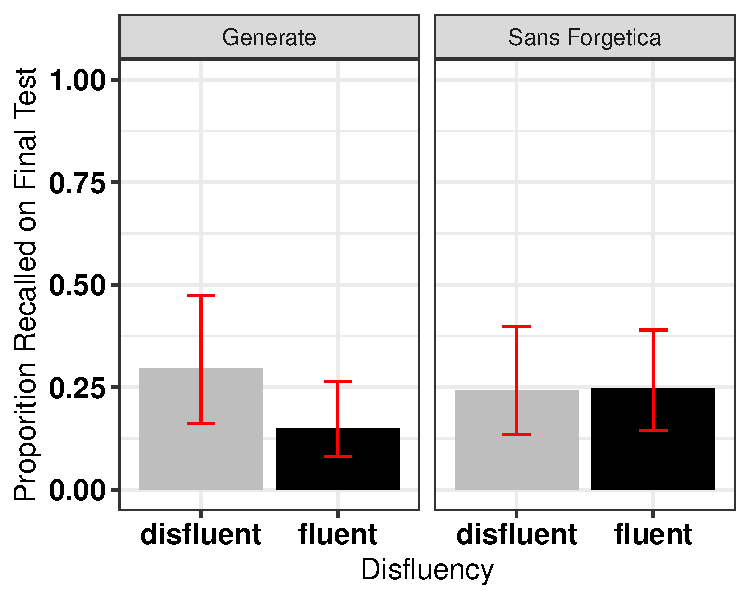
\includegraphics{SF_Paper_draft_files/figure-latex/unnamed-chunk-1-1.pdf}

\begin{Shaded}
\begin{Highlighting}[]
\NormalTok{ls1 <-}\StringTok{ }\KeywordTok{emmeans}\NormalTok{(a1, }\KeywordTok{c}\NormalTok{(}\StringTok{"dis"}\NormalTok{), }\DataTypeTok{by=}\StringTok{"condition"}\NormalTok{) }\CommentTok{# get the simple effects test for signifcant interaction. }

\CommentTok{#pairwise comparison}
\NormalTok{flex1=}\KeywordTok{pairs}\NormalTok{(ls1)}

\KeywordTok{kable}\NormalTok{(flex1)}
\end{Highlighting}
\end{Shaded}

\begin{longtable}[]{@{}llrrrrr@{}}
\toprule
contrast & condition & estimate & SE & df & t.ratio &
p.value\tabularnewline
\midrule
\endhead
disfluent - fluent & Generate & 0.1339080 & 0.0184121 & 230 & 7.2728251
& 0.0000000\tabularnewline
disfluent - fluent & Sans Forgetica & -0.0025797 & 0.0184121 & 230 &
-0.1401076 & 0.8886976\tabularnewline
\bottomrule
\end{longtable}

\hypertarget{experiment-2}{%
\section{Experiment 2}\label{experiment-2}}

\textless{}\textless{}\textless{}\textless{}\textless{}\textless{}\textless{}
HEAD Experiment 2 examined the SF in a more educatioanlly realistic
scenairo. We presented participants a passage on ground water where some
of the material was either: pre-highlighted, presented in SF, or
presneted with no changes. This was a between-subjects manipulation.
Specifically participants read a passage about ground water (856 words)
from the U.S. Geological Survey website (Yue, Storm, Kornell, Bjork,
2014). Eleven critical phrases \footnote{orginally we had 12 critical
  phrases but a pilot test after the pregreistation showed that one of
  the questions was repeated twice so we removed one of them and also
  added a manipulation check question to sure participants were paying
  attention} each containing a different keyword, were selected from the
passage (e.g., the term \emph{recharge} was the keyword in the phrase:
Water seeping down from the land surface adds to the ground water and is
called recharge water.) and were either presented in SF, highlighted, or
unchanged. Then, 11 fill-in-the blank questions were created from these
phrases by deleting the keyword and asking participants to provide it on
the final test (e.g., Water seeping down from the land surface adds to
the ground water and is called \_\_\_\_\_\_\_\_\_\_ water).

\hypertarget{particiapnst-were-recruited-from-the-sona-pool.-data-was-collected-data-until-the-end-of-the-fall-semester-2019-and-we-ended-up-with-545-ps-181-in-the-highlight-condition-182-in-the-normal-condition-and-182-in-the-passage-condition.-we-preregistered-a-sample-size-of-510-participants-170-per-group-to-detect-a-small-to-medium-effect-d-.35-with-90-power.}{%
\section{Particiapnst were recruited from the SONA pool. Data was
collected data until the end of the Fall semester 2019 and we ended up
with 545 Ps (181 in the Highlight condition, 182 in the Normal
condition, and 182 in the Passage condition). We preregistered a sample
size of 510 participants (170 per group) to detect a small-to medium
effect (d = .35) with 90\%
power.}\label{particiapnst-were-recruited-from-the-sona-pool.-data-was-collected-data-until-the-end-of-the-fall-semester-2019-and-we-ended-up-with-545-ps-181-in-the-highlight-condition-182-in-the-normal-condition-and-182-in-the-passage-condition.-we-preregistered-a-sample-size-of-510-participants-170-per-group-to-detect-a-small-to-medium-effect-d-.35-with-90-power.}}

Experiment 2 examined the SF in a more educatioanlly realistic scenairo.
We presented participants a passage on ground water where some of the
material was either: pre-highlighted, presented in SF, or presneted with
no changes. This was a between-subjects manipulation. Specifically
participants read a passage about ground water (856 words) from the U.S.
Geological Survey website (Yue, Storm, Kornell, Bjork, 2014). Eleven
critical phrases \footnote{orginally we had 12 critical phrases but a
  pilot test after the pregreistation showed that one of the questions
  was repeated twice so we removed one of them and also added a
  manipulation check question to sure participants were paying attention}
each containing a different keyword, were selected from the passage
(e.g., the term \emph{recharge} was the keyword in the phrase: Water
seeping down from the land surface adds to the ground water and is
called recharge water.) and were either presented in SF, highlighted, or
unchanged. Then, 11 fill-in-the blank questions were created from these
phrases by deleting the keyword and asking participants to provide it on
the final test (e.g., Water seeping down from the land surface adds to
the ground water and is called \_\_\_\_\_\_\_\_\_\_ water).

We collected data until the end of the Fall semester 2019 and ended up
with 545 Ps (181 in the Highlight condition, 182 in the Normal
condition, and 182 in the Passage condition). We preregistered a sample
size of 510 participants (170 per group) to detect a small-to medium
effect (d = .35) with 90\% power.

\begin{verbatim}
## [1] "/Users/gellr/SF_Expt2"
\end{verbatim}

\begin{verbatim}
## Warning: Missing column names filled in: 'X1' [1]
\end{verbatim}

\begin{verbatim}
## Warning: Duplicated column names deduplicated: 'X1' => 'X1_1' [7]
\end{verbatim}

\begin{Shaded}
\begin{Highlighting}[]
\NormalTok{a1 <-}\StringTok{ }\KeywordTok{aov_ez}\NormalTok{(}\StringTok{"ResponseId"}\NormalTok{, }\StringTok{"acc"}\NormalTok{, scored_ground_aov, }
             \DataTypeTok{between =} \KeywordTok{c}\NormalTok{(}\StringTok{"Passage"}\NormalTok{)) }\CommentTok{# one way}
\end{Highlighting}
\end{Shaded}

\begin{verbatim}
## Converting to factor: Passage
\end{verbatim}

\begin{verbatim}
## Contrasts set to contr.sum for the following variables: Passage
\end{verbatim}

\begin{Shaded}
\begin{Highlighting}[]
\CommentTok{#plot the results}

\KeywordTok{kable}\NormalTok{(}\KeywordTok{nice}\NormalTok{(a1))}
\end{Highlighting}
\end{Shaded}

\begin{longtable}[]{@{}llllll@{}}
\toprule
Effect & df & MSE & F & ges & p.value\tabularnewline
\midrule
\endhead
Passage & 2, 541 & 0.07 & 3.27 * & .01 & .04\tabularnewline
\bottomrule
\end{longtable}

\begin{Shaded}
\begin{Highlighting}[]
\NormalTok{ls1 <-}\StringTok{ }\KeywordTok{emmeans}\NormalTok{(a1, }\DataTypeTok{specs =} \StringTok{"Passage"}\NormalTok{ ) }\CommentTok{# get the simple effects test for signifcant interaction. }

\NormalTok{flex1=}\KeywordTok{summary}\NormalTok{(}\KeywordTok{pairs}\NormalTok{(}\KeywordTok{emmeans}\NormalTok{(a1, }\DataTypeTok{specs=}\StringTok{"Passage"}\NormalTok{)))}

\NormalTok{flex1}\OperatorTok{$}\NormalTok{d =}\StringTok{ }\NormalTok{flex1}\OperatorTok{$}\NormalTok{estimate }\OperatorTok{/}\StringTok{ }\KeywordTok{sqrt}\NormalTok{(a1}\OperatorTok{$}\NormalTok{anova_table}\OperatorTok{$}\NormalTok{MSE)}

\KeywordTok{kable}\NormalTok{(flex1)}
\end{Highlighting}
\end{Shaded}

\begin{longtable}[]{@{}lrrrrrr@{}}
\toprule
contrast & estimate & SE & df & t.ratio & p.value & d\tabularnewline
\midrule
\endhead
Highlight - Normal & 0.0714965 & 0.0282951 & 541 & 2.5268165 & 0.0315955
& 0.2656131\tabularnewline
Highlight - SF & 0.0451158 & 0.0282562 & 541 & 1.5966697 & 0.2479288 &
0.1676075\tabularnewline
Normal - SF & -0.0263807 & 0.0282562 & 541 & -0.9336249 & 0.6192373 &
-0.0980056\tabularnewline
\textgreater{}\textgreater{}\textgreater{}\textgreater{}\textgreater{}\textgreater{}\textgreater{}
12407944d8d1c & b604995f74327 & fa48b5913659 & 0f & & &\tabularnewline
\bottomrule
\end{longtable}

\begin{verbatim}
## [1] "/Users/gellr/SF_Expt2"
\end{verbatim}

\begin{verbatim}
## Warning: Missing column names filled in: 'X1' [1]
\end{verbatim}

\begin{verbatim}
## Warning: Duplicated column names deduplicated: 'X1' => 'X1_1' [7]
\end{verbatim}

\begin{longtable}[]{@{}llllll@{}}
\caption{Table 2.Pairwise Comparisons}\tabularnewline
\toprule
Effect & df & MSE & F & ges & p.value\tabularnewline
\midrule
\endfirsthead
\toprule
Effect & df & MSE & F & ges & p.value\tabularnewline
\midrule
\endhead
Passage & 2, 541 & 0.07 & 3.27 * & .01 & .04\tabularnewline
\bottomrule
\end{longtable}

\begin{longtable}[]{@{}lrrrrrr@{}}
\toprule
contrast & estimate & SE & df & t.ratio & p.value & d\tabularnewline
\midrule
\endhead
Highlight - Normal & 0.0714965 & 0.0282951 & 541 & 2.5268165 & 0.0315955
& 0.2656131\tabularnewline
Highlight - SF & 0.0451158 & 0.0282562 & 541 & 1.5966697 & 0.2479288 &
0.1676075\tabularnewline
Normal - SF & -0.0263807 & 0.0282562 & 541 & -0.9336249 & 0.6192373 &
-0.0980056\tabularnewline
\bottomrule
\end{longtable}

\includegraphics{SF_Paper_draft_files/figure-latex/unnamed-chunk-6-1.pdf}
We found that infromation that was pre-hightlighted had better recall
than passages presentened normally. We did not find that passages in SF
were better remembered than normal or highligheted passages.

\hypertarget{conclusions}{%
\section{Conclusions}\label{conclusions}}

The evidence contained herein suggests that SF does not have the
mnemonic effects pruported by its creators. Now it is possible that
there is an effect of SF, but the effect size might be smaller than we
could detect acorss our two studies. Our SESOI was d = .35. If so, it
probably does not have any real educational benefit. It is our
conclsuion that SF is really forgetable and you should not be using it
as a way to boost leanring.

\end{document}
